\documentclass[12pt, oneside]{report}
\usepackage[
backend=bibtex8,
style=ieee,
citestyle=numeric
] {biblatex}
\usepackage[top=2in,bottom=1in,right=1in,left=1in]{geometry}
\usepackage[document]{ragged2e}
\usepackage{setspace}
\usepackage{titlesec} % for formatting the chapter titles
\usepackage{graphicx}
\usepackage[titletoc,title]{appendix}
\usepackage{wrapfig}
\usepackage[font=small]{caption, subcaption}
\usepackage{hyperref}
\usepackage[table,xcdraw]{xcolor}

% Font packages and settings
\usepackage{fontspec}

\titleformat{\chapter}[block]
{\normalfont\huge\bfseries}{\thechapter}{20pt}{}
\titlespacing*{\chapter}
{0pt}{20pt}{20pt}
\setcounter{tocdepth}{2}
\setcounter{secnumdepth}{2}
\setlength{\parindent}{1cm}
\setmainfont{Times New Roman}
\doublespacing
\addbibresource{citations.bib}

\begin{document}
	\thispagestyle{empty}
	\pagenumbering{roman}

	\begin{center}
		\singlespacing
		\vspace{4in}
		THESIS TITLE\\
		\vspace{1in}
		Jacob Timothy Hill\\
		\vspace{1in}
		A dissertation submitted to the faculty at the University of North Carolina at Chapel Hill in partial fulfillment of the requirements for the degree of Doctor of Philosophy in the School of Information and Library Science.\\
		\vspace{1in}
		Chapel Hill\\
		2020
		\vspace{1in}
	\end{center}
	\begin{raggedleft}
		Approved By:\\
		Ryan Shaw\\
		Melanie Feinberg\\
		Jaime Arguello\\
		Omid Ghaemmagami\\
		Ted Underwood\\
	\end{raggedleft}
\newpage
\begin{center}
	\vspace*{\fill}
	\copyright 2020\\
	Jacob Timothy Hill\\
	ALL RIGHTS RESERVED
	\vspace{1in}
\end{center}
\newgeometry{top=2in,bottom=1in,right=1in,left=1in}
\begin{center}
	\textbf{ABSTRACT}
\end{center}
\newgeometry{margin=1in}
\setlength{\parindent}{15pt}
\tableofcontents
\newpage
\listoffigures
\chapter{Introduction}
\pagenumbering{arabic}
Overall argument: We are applying algorithms developed for information science and computer science tasks to humanities tasks and this is problematic because it requires significantly more interrogation of the process, the bias in the data (text encoding, archival bias e.g. whats included and not included, etc.).

When moving into a new field like digital humanities it is important to explore some questions related to methodological fit. These explorations have to be done for different fields and different problems. We can't have one solution for all humanities problems. The kind of work done thus far relates to some basic explorations of the application of algorithms to humanities problems, often without a clear idea of how to interpret the results, as well as some NLP work that addresses issues related to Arabic and Persian corpora. Before applying NLP problems to Bah\'{a}'\'{i} texts it is important to contextualize the problems which entails framing them in such a way that computer scientists and humanists, to adopt an overly simplistic schema of the audience, can engage in a common conversation.

Need evaluation methods that take into consideration the basic “quality” of the word vectors without losing site of the object of interest.

\chapter{Literature Review}

\chapter{The Linguistic Setting}
\par
Among the challenges in applying algorithms developed by computer and information scientists to humanities problems is that there is an, often unnoticed or underappreciated, shift in context that requires reckoning.
In machine learning research the data set and evaluation methods are generally treated as controlled variables or benchmarks for testing algorithms.
In humanities research the data set---the use of language within a given social and historical context---is the thing of interest.
A simple inversion of this relationship (treating the algorithms as controlled variables and substituting data sets) could lead to significant problems.
This is the likely point of departure for most humanists in learning to program and examine old problems through new lenses but it cannot be the standard for digital humanities research.
It must, in time, give way to a more careful inquiry into the inputs, transformations, and outputs of each step in the algorithm.
\par
Humanists must begin to think more like computer scientists.
They must learn to deconstruct algorithms into their common components and understand how and why these components are recycled and exchanged to build new algorithms.
These skills are required in order to know which algorithms to apply to a given problem and how subtle changes might impact the results in significant ways.
They must also learn to apply humanist techniques towards an interrogation of the processes through which their data came to be---historical, cultural, political processes that might have significant bearing on the choice of algorithms.
\par
The problem articulated above can be more succinctly described as a need for local language models in humanities research.
Language can change in meaningful ways across time, place, and storage medium.
These changes need to be accounted for in computational linguistics research.
In computer science articles they are often considered in detail when a data set is initially prepared and then relegated to a footnote thereafter, never to be considered again.
This is perfectly reasonable given the interest of computer scientists in algorithm design.
But humanists are frequently in the position of constructing new, or refactoring existing, datasets and exploring these datasets through the lenses of various algorithms.
At times they may need to change existing algorithms or tune parameters in order to apply them to new ends.
To do so safely an account of the data set and algorithms must be given, an account that enables readers to peer into the often invisible sequence of decisions that led to the reported results.
\par
The current chapter aims to articulate some of the complexities of the Arabic and Persian language as well as the Bah\'{a}'\'{i} writings.
Many of the former are well known to computational linguists who work with these languages.
Some of the latter will also be known to Bah\'{a}'\'{i} scholars well read in the core writings of the Bah\'{a}'\'{i} Faith.
No attempt has been made, however, to mediate the two worlds.
There are no Bah\'{a}'\'{i} scholars using computational linguistics as a research methodology, nor any information or computer scientists using computational linguistics to improve access and discovery.
\par
The Bah\'{a}'\'{i} writings are something of a linguistic anomaly in that, within the corpus of a single author, the style of writing, the use of language, can shift dramatically from one text to another, even within a single text.
The writings of Bah\'{a}''u'll\'{a}h exhibit this characteristic throughout.
Few writers have such a wide ranging audience in mind or adapt so much to the linguistic biases of their audience.
Bah\'{a}''u'll\'{a}h's writings sway between elevated Arabic and vernacular Persian, touching upon everything in between, and often branching out more substantially into something that might be recognized as a distinct literary genre.
In some instances His literary works are unsolicited.
More often than not, however, His style and choice of words is the result of deference to the sensitivities of the recipient of the text; they are an answer to a question or request.
This context must be borne in mind when selecting algorithms and evaluating their results.
\section{The ``Raw'' Data}
\par
The sample of Bah\'{a}'\'{i} writings used in this study consists of nearly everything available on the authorized website of the Universal House of Justice (www.reference.bahai.org)---the elected governing body of the international Bah\'{a}'\'{i} community---with the exception of some early scholarly attempts to compile the Bah\'{a}'\'{i} writings, such as those of `Abdu'l-Ham\'{i}d Ishr\'{a}q-Kh\'{a}vari, and a few other largely derivative compilations.
Including the former would require significant manual labor to separate the words of the author from the passages of Bah\'{a}'\'{i} scripture he compiles.
Including the latter would add duplicate text, possibly skewing the results of the study through the multiplication of commonly occurring passages.
Volumes consisting of scanned images without machine readable text were naturally excluded because of the significant work required to prepare them for computation.
For a list of all published volumes included in the present study see \nameref{app-1}.
For a relational view of the number of works in the sample compared to all extant works see \autoref{fig:works-table}.
\begin{figure}[htb]
\centering
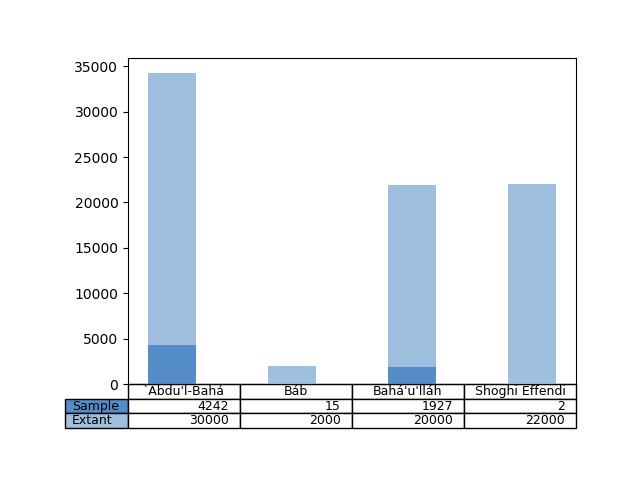
\includegraphics[width=15cm]{figures/works-table.png}
\caption[Bah\'{a}'\'{i} works sampled relative to all extant works]{Bah\'{a}'\'{i} works sampled relative to all extant works}
\label{fig:works-table}
\end{figure}
\par
The individual Bah\'{a}'\'{i} works were parsed from the published volumes listed in \nameref{app-1} and labeled with author and language (Arabic or Persian).
This binary linguistic labeling at the level of the work may be somewhat misleading given the fluidity of language that is characteristic of the Bah\`{a}'\'{i} writings.
A more granular labeling strategy---say at the level of the sentence or paragraph---though ideal, would require an unreasonable increase in manual labor.
By way of compromise, the works labeled `Arabic' are fully Arabic.
The occasional Persian word, or Persianized Arabic word, may slip in but the general structure is Arabic.
There are no Persian sentences, prepositions, or pronouns.
Works were labeled manually, checked computationally, reinspected and relabeled when necessary.
The checking step consisted of generating a list of high frequency Persian words, which included all prepositions and pronouns, and iteratively searching each Arabic text for words in this list.
If the Arabic text contained any of the high frequency Persian words, it was reinspected and, if necessary, relabeled.
\par
This labeling strategy is justified by historical and cultural precedent.
Persians, being largely Muslim, were expected to have some knowledge of the Arabic language---the language of the Qur'\'{a}n.
Arab Muslims had no motivation to learn Persian, except the minority who lived in Iran.
The impact of this cultural and historical phenomenon on the Bah\'{a}'\'{i} corpus is discernible in the larger number of wholly Arabic works---particularly among earlier authors---as well as the frequency of lengthy Arabic passages in most Persian works.
There are a significant number of Persian works without Arabic passages, but given the expectation that Persian readers would know some Arabic, the appearance of large segments of Arabic text in Persian works is commonplace.
\par
The implications of such a strategy are that the total number of Arabic and Persian words are skewed towards Persian (there are 706,426 Arabic words compared to 1,906,607 Persian).
Most of the ``Persian'' works contain large sections of Arabic text which gets counted in the Persian word count.
This, unfortunately, is unavoidable given that a more granular labeling approach is not presently feasible.
\par
In order to provide context, a large corpus of contemporary texts were selected for comparison, which included a collection of over 60,000 Persian poems (``and a few prose texts'') prepared by the Persian Digital Library (PDL) Pilot Project \cite{noauthor_persian_nodate} and nearly 350 lengthy Arabic works from the `Knowledge, Information Technology and the Arabic Book' (KITAB) \cite{maxim_romanov_openiti:_2019} project.
The selections from the KITAB project were limited to works from the 12th-14th centuries AH (October 26, 1688-November 21, 1979) which is roughly contemporaneous with the Bah\'{a}'\'{i} works sampled.
All works in the PDL corpus were added without exception while works in the KITAB corpus that contained Persian passages were removed to maintain consistency with the linguistic labeling strategy applied to the Bah\'{a}'\'{i} corpus.
\section{Side Effects of Text Encoding}
\par
All computational linguistic work requires some level of preprocessing.
However, there are several considerations that are peculiar to languages written in a modified form of the Arabic script.
One such consideration is the existence of ambiguous characters---characters with the same form, but different encodings \cite{jaf_semi-automatic_2016}---that stem from decisions made about how each language should be encoded.
These characters appear the same to the human eye but have different underlying encodings.
What appears to be the same letter in Persian and Arabic---the letter ك \textit{k\`{a}f} for example---may in fact be two distinct encodings.
These ambiguous characters must be normalized during preprocessing.
Failure to conflate ambiguous characters results in the proliferation of vocabulary; a significant number of words that appear the same to the reader and were intended to be the same by the writer are treated as different words by the computer.
Failure to remediate this issue prior to any down stream tasks can have significant negative effects on the outcome of those tasks.
\begin{wrapfigure}{r}{.5\textwidth}
	\begin{minipage}{\linewidth}
		\centering\captionsetup[subfigure]{justification=centering}
		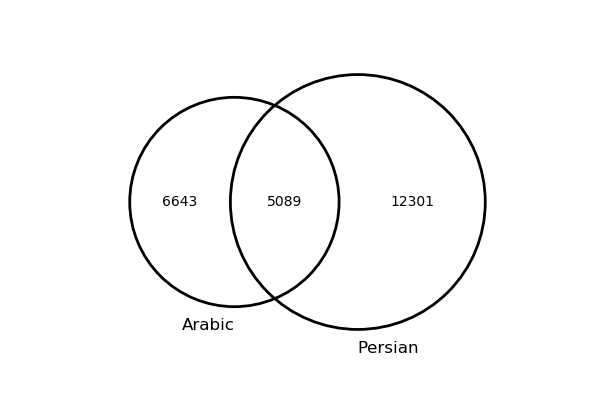
\includegraphics[width=\linewidth]{figures/venn-proc-one-freq5.png}
		\subcaption{}
		\label{fig:char-norm-a}\par\vfill
		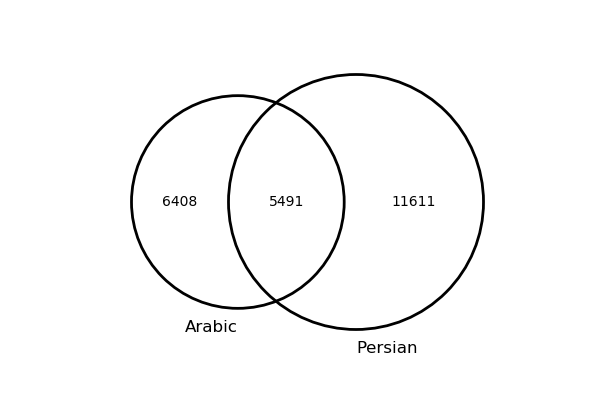
\includegraphics[width=\linewidth]{figures/venn-proc-two-freq5.png}
		\subcaption{}
		\label{fig:char-norm-b}
		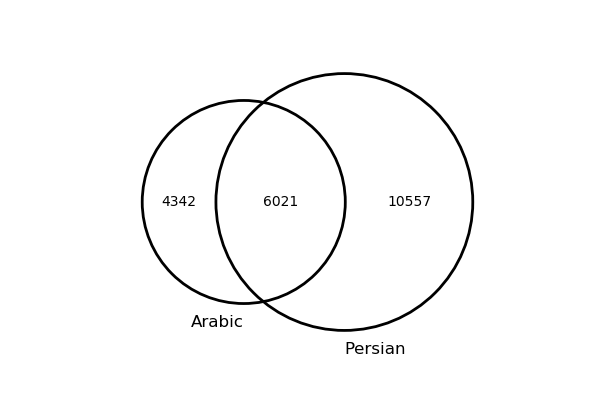
\includegraphics[width=\linewidth]{figures/venn-proc-three-freq5.png}
		\subcaption{}
		\label{fig:char-norm-c}
	\end{minipage}
	\caption[Venn diagrams depicting the effects of various processing decisions]{Arabic and Persian vocabulary with various levels of processing}\label{fig:char-norm}
\end{wrapfigure}
These effects can be especially consequential if the researcher is interested in the interactions across two languages written in the Arabic script given that the shared vocabulary---the loan words shared between languages that evince centuries of linguistic and cultural exchange---are obscured by the historical processes through which the languages were encoded.
\par
Another issue affecting languages written in Arabic script is the inconsistent use of diacritical marks.
In Arabic and Persian short vowels were historically not written, though they are pronounced in speech.
The reader is expected to know when to add the vowels, and which ones to add.
There are, of course, a significant number of homographs which led to the subsequent development of diacritical marks that could be optionally added above or below letters to specify the following short vowel and thereby remove any ambiguity.
Adoption has not been consistent, however, which compounds the vocabulary proliferation problem described above.
These too must be removed to avoid diluting the statistic signal.
\par
A number of steps were taken to remediate this issue, the effects of which are summarized in \autoref{fig:char-norm}.
For all steps, the minimum frequency threshold was set at five; words that occur less than five times across the whole corpus were removed.
Diagram (a) shows the respective vocabulary with no data cleaning.
Diagram (b) shows results after several language-agnostic cleanup steps were taken.
Punctuation marks were removed as well as characters that produce only visual effects, such as spaces, tabs, and newline characters.
Diagram (c) shows the results of removing character disambiguation and diacritical marks in addition to the steps taken in (b).
\par
The term ``preprocessing'', commonly used to describe this kind of work gives some indication of the level of importance it is given in the literature.
Though it is deemed essential to any downstream task, in most computational linguistic research it is briefly described, or not at all.
The computer science research community trends towards standardizing these practices and moving on to other, more interesting, questions.
Precedent often trumps rationale in determining which data cleaning steps are taken, and with good reason.
Precedent has worked fine for decades and the circumstances have not changed.
Moreover, the consistency of data across papers enables researches to quickly compare the results of one algorithm to another and home in on the effects of the novel algorithm.
The application of computational linguistics strategies to humanities problems---problems they were not overtly designed to solve---warrants a re-examination and justification of these steps, as does the application to non-western languages.
Each of these contextual changes introduces opportunities for confusion.
\par
The Venn diagrams in \autoref{fig:char-norm} provide insight into the effects preprocessing decisions can have.
As is expected, without any intervention (a) there is a significant overlap in vocabulary.
After all, many of the Persian texts contain Arabic passages and Persian, in general, is riddled with Arabic vocabulary.
Language agnostic processing steps reduced the total vocabulary by 2.2\% (523 words), the Arabic vocabulary by 3.5\% (235 words), and the Persian vocabulary by 5.6\% (690 words), while the intersection increased by 7.9\% (402 words).
Removing diacritical marks and conflating ambiguous characters reduced the total vocabulary by an additional 11\% (2,590 words), the Arabic vocabulary by 32\% (2,066 words), and the Persian vocabulary by 9.1\% (1,045 words), while increasing the intersecting vocabulary by 9.7\% (530 words).
The reduction in vocabulary consisted exclusively of non-existent words---side effects of the text encoding process or variances in typography.
\par
It is worth noting, also, the effect the minimum frequency threshold has on vocabulary.
One of the of implications of Zipf's law is the common existence of a long tail of words that occur only once, or a few times.
Removing these words helps to speed up computation and reduce noise; words that occur only once can have no interaction effects and words that occur only a few times do not provide enough data to draw statistically significant conclusions.
With no preprocessing 243,639 words were removed, with language agnostic preprocessing only 163,692 words were removed, and with language agnostic processing, removal of diacritical marks and conflation of ambiguous characters only 103,824 words were removed.
The trend towards discarding fewer words with each step of processing is a clear indication of the efficacy of these techniques; nearly 140,000 words were sparred from removal, each one boosting the signal of a legitimate word in the corpus.
The raw count is not an adequate appraisal of the value of these techniques, however.
Considering the ultimate objective of representing this vocabulary as a single matrix, these ~140,000 words take on added significance.
\par
To illustrate this point and simultaneously delineate the limitations of the adopted strategies consider the word كلمة \textit{kalima}, an Arabic loan word frequently used in Persian.
The first letter ك \textit{`kaf`} has a different encoding in Arabic and Persian systems.
Given that text encoding is not well understood by your average typist and considering that many of these typists may know Arabic and Persian and use both keyboards the word will bifurcate in both languages resulting in two forms in each language.
This word has a further problem with its final letter.
In the Arabic original form it ends in ة \textit{t\'{a}ʾ marb\'{u}ta}, a letter indicating the feminine gender of the word.
This letter is not found in Persian and is replaced by the letter ه \textit{heh}, a somewhat similar looking letter that also exists in Arabic.
The addition of this variable results in four different possible forms for the same word:
\begin{enumerate}
	\item Arabic ك \textit{`kaf`}... ة \textit{t\'{a}ʾ marb\'{u}ta},
	\item Persian ک \textit{`kaf`}... ه \textit{heh},
	\item Arabic ك \textit{`kaf`}... ه \textit{heh},
	\item Persian ک \textit{`kaf`}... ة \textit{t\'{a}ʾ marb\'{u}ta}.
\end{enumerate}
Normalizing the ك \textit{`kaf`} would eliminate forms 2 and 4.
For many words this step would completely remove the problematic effects of divergent text encodings.
Unfortunately, there is no easy solution for the ه \textit{heh} ending adopted in Persian.
Since it is used in Arabic, and often at the end of words, it cannot be blindly replaced with a ة \textit{t\'{a}ʾ marb\'{u}ta}.
This strategy would fix words like كلمة \textit{kalima} while creating other problems in the process.
Normalizing variant text encodings is only a solution for vocabulary proliferation problems resulting from the historical circumstances of text encoding in Arabic and Persian.
It cannot solve problems resulting from other historical processes, such as those responsible for the substitution of the t\'{a}ʾ marb\'{u}ta with the heh.
\par
The above example demonstrates how failure to adequately prepare language data for down stream tasks can delegitimize the outcome of those tasks.
Meaningless sequences of encodings will erroneously be treated as words and examined for statistical significance while meaningful words will be discarded.
While the need for preprocessing is likely understood to even novice digital humanists, the need for local processing models is likely unclear to many.
Global language models---one size fits all approaches---can be problematic in unexpected ways.
Languages have developed through unique historical and cultural circumstances.
They have been transferred from analogue to digital form through different processes.
Failure to adequately understand and account for the historical processes in which the language developed and was encoded for computational processing can undermine the whole process.
\section{Peculiarities of Language and Literary Products}
\par
The discussion above demonstrates some problems that stem from the history of encoding languages in Arabic script for computation. Failure to resolve these issues can result in undesirable donwstream effects. Text encoding is not the only historical process with implications for computational linguistics. Language and literature are both products of history. These products are a part of the context that must be accounted for in digital humanities research. Consider, for example, the field of stylometry that has proven fruitful for author recognition and other problems in literary research.
\par
There is a natural temptation to turn to stylometry for evidence of Bah\'{a}'u'llah's writing style in relation to other authors but these methods are often not applicable across language.
For example, the most frequently used stylometric methods---average sentence length, average word length \cite{justin_rice_what_2018}, lexical richness (the proportion of unique words to total words \cite{justin_rice_what_2018}), and the chi-squered method---each pose problems in Arabic and Persian.
Justin Rice uses average sentence length as a metric to distinguish the style of Hemingway's writings from that of other writers \cite{justin_rice_what_2018}.
In classical Arabic and Persian, however, the period is an afterthought.
It is used inconsistently when it is used at all and it must, until proven otherwise for each text, be treated as what Gennete refers to as `paratextuality'–--an element outside of the text that influences its reading \cite{genette_gerard_palimpsests:_1997}.
Periods in English, and often in modern Arabic and Persian, are part of the author's literary production; they are added by the author and can be used as evidence of his or her writing style.
In the writings of Bah\'{a}'u'llah periods were added by scribes or publishers, if at all, and cannot therefore be used as evidence of writing style.
Without periods there is no reliable way of determining sentence length which makes this metric unsuitable for the most research in Arabic and Persian.
Given that the full stop is becoming more common in modern literature, there may be some exceptions to this rule.
\par
The other three metrics have been used as a means of author detection and, cautiously, to measure the writing ability of authors, the assumption being that there is a correlation between these statistics and a writer's knowledge of the language.
In some cases word length has been combined with other language specific data resulting in more effective models for specific circumstances.
For example, Renjui and Chu combine word length with word-final tone motifs and segment-final motifs to improve author detection in Chinese texts \cite{renkui_stylometric_nodate}.
In Arabic, each of these methods will be affected by formatting inconsistencies related to the particle `waw', a single letter meaning `and', which is frequently found in all Arabic writing.
Using `waw' frequently would not have the same effect in Arabic as the frequent use of `and' in English.
The former is perfectly acceptable, whereas, the latter would be considered poor style.
Given the lack of punctuation in classical Arabic the `waw' filled the same role as the English `and', `comma', and `full stop'.
The problem for determining word length is that the `waw' is inconsistently adjoined with the succeeding word without a space in between them.
Thus instead of having many words of length one, a significant number of occurrences are merged with the following word.
This, like the oxford comma in English, could be an effect of either author style or a side effect introduced when the physical text was made digital.
This is consistently the case with the writings of the B\'{a}b sampled here \autoref{fig:word-length-bab}---there are no words of length one---and inconsistently the case with the writings of al-Shaykh Murtaḍ\'{a} al-\'{A}ns\'{a}r\'{i} \autoref{fig:word-length-murtada-ansari}, indicating, probably, the compilation of his writings from different sources.
The full extent to which this will impact these metrics is unclear and beyond the scope of this study.
At the very least it would inflate word lengths, diminish word counts, and skew lexical richness through the addition of many false words.
These effects would be inconsistent across author, making comparative inquiries particularly risky.
\par
Another way in which the Arabic language challenges all down stream tasks is through notoriously intractable tokenization.
In English, and most Western languages, dealing with punctuation and splitting on white space is sufficient to segment larger chunks of text into tokens.
Tokenization is much more complicated in Arabic due to its morphological complexity which is realized through ``concatenative (affixes and stems) and templatic (root and patterns) morphology \cite{habash_arabic_2006}.''
More importantly, tokenization techniques are domain dependent; if the test set differs from the training set, the tokenizer will perform poorly \cite{sajjad_challenging_2017}, \cite{habash_arabic_2006}.
This is particularly ominous for those working with the Bah\'{a}'\'{i} writings; given that the style of writing can change in so many unanticipated ways, constructing a training set that is representative of the entire corpus would be a major undertaking.
The inconsistent spelling of certain characters–--variants of Hamzated Alif, أ or إ are frequently written without their Hamza (ء)---further complicates tokentization by increasing ``sparsity (multiple forms of the same word) and ambiguity (same form corresponding to multiple words) \cite{habash_arabic_2006}.''
These characteristics could impact word counts and metrics that build on them such as lexical richness and chi-squared and, as in the case of the `waw' problem described above, would add increased risk in comparative studies between corpora from different domains or that have been digitized and compiled through different processes.
One would need to take added precautions to investigate the history of the corpora and somehow account for the impact inconsistent tokenization performance might have on the process in order to avoid drawing unwarranted or misleading conclusions from tokenization inconsistencies between corpora.
A quick comparison of the word length data on Bah\'{a}'u'llah \autoref{fig:word-length-bahaullah} with that of the B\'{a}b \autoref{fig:word-length-bab} and `Abdu'l-Bah\'{a} \autoref{fig:word-length-abdulbaha} can illustrate this point.
\begin{figure}[htb]
	\centering
	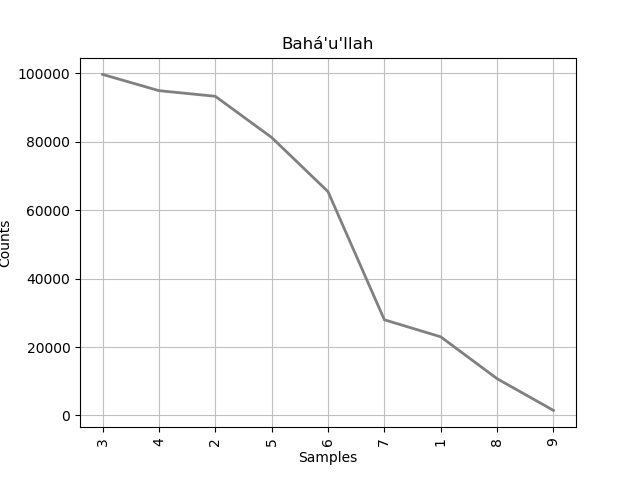
\includegraphics[width=15cm]{figures/word-length-bahaullah.png}
	\caption[Most common word lengths used by Bah\'{a}'u'llah]{Most common word lengths used by Bah\'{a}'u'llah}
	\label{fig:word-length-bahaullah}
\end{figure}
\par
The trends for the first two are similar with the exception that one letter words do not occur in the writings of the B\'{a}b.
This is certainly not attributable to writing style.
It is not possible to write prose in Arabic without the use of the `waw'.
Given that the entire corpus of the B\'{a}b used in this study was published in a single volume, this is likely a feature of the digitization process.
It is unclear how this text was transferred from its physical form to the digital version used in this study but it was likely typed by one or more individuals who chose not to add spaces after the `waw'.
\par
The latter two authors trend towards longer words.
This could be evidence of the relative levels of education each received.
`Abdu'l-Bah\'{a} did not have much in the way of formal schooling but He served as a scribe for His father, Bah\'{a}'u'llah, and would have received some training through this service.
Moreover, a cursory review of some of `Abdu'l-Bah\'{a}'s writings such as `Some Answered Questions' \cite{abdul-baha_answered_1990} and His talks in the west published in `Abdu'l-Bah\'{a} in London' \cite{abdul-baha_abdul-baha_1982}, `Paris Talks' \cite{abdul-baha_paris_nodate}, and `Promulgation of Universal Peace' \cite{abdul-baha_promulgation_1982} indicates that He was well read and conversant in many topics familiar to educated westerners.
\begin{figure}[htb]
	\centering
	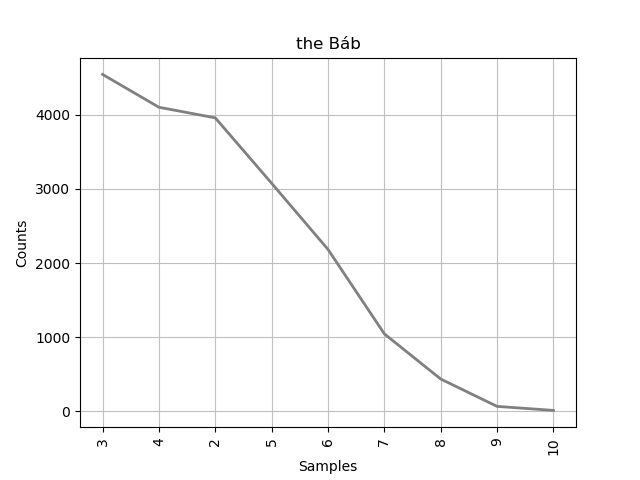
\includegraphics[width=15cm]{figures/word-length-bab.png}
	\caption[Most common word lengths used by the B\'{a}b]{Most common word lengths used by the B\'{a}b}
	\label{fig:word-length-bab}
\end{figure}
\begin{figure}[htb]
	\centering
	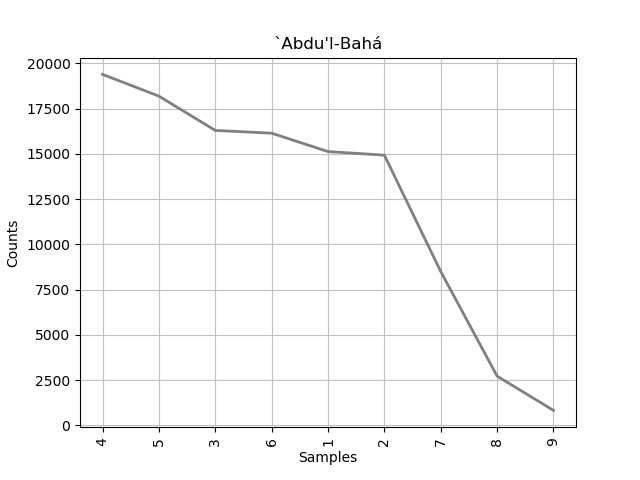
\includegraphics[width=15cm]{figures/word-length-abdulbaha.png}
	\caption[Most common word lengths used by `Abdu'l-Bah\'{a}]{Most common word lengths used by `Abdu'l-Bah\'{a}}
	\label{fig:word-length-abdulbaha}
\end{figure}
\par
Al-Shaykh Murtaḍ\'{a} al-\'{A}ns\'{a}r\'{i}, who has been referred to as \autoref{fig:word-length-murtada-ansari}–``the most influential mujtahid of his time whose supremacy was acknowledged also by Turkish, Arab, and Indian Sh\'{i}'\'{i}s \cite{abd_al-hadi_hairi_shiism_1977}'', and who was a contemporary of all three Authors in question, was certainly well educated in the traditional sense.
His writing also trends toward longer words.
\begin{figure}[htb]
	\centering
	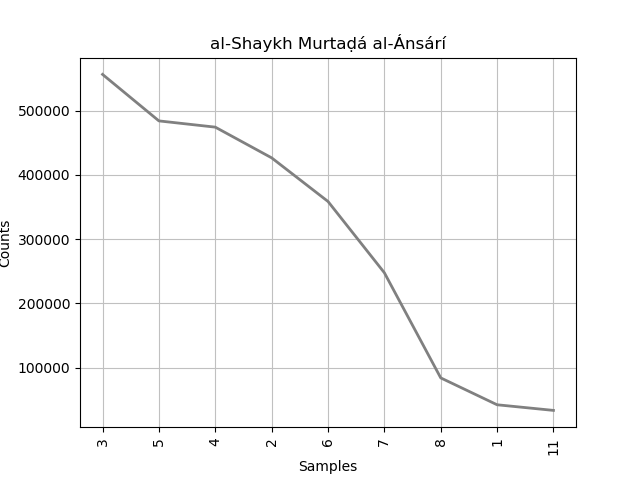
\includegraphics[width=15cm]{figures/word-length-shaykh-murtada.png}
	\caption[Most common word lengths used by al-Shaykh Murtaḍ\'{a} al-\'{A}ns\'{a}r\'{i}]{Most common word lengths used by al-Shaykh Murtaḍ\'{a} al-\'{A}ns\'{a}r\'{i}}
	\label{fig:word-length-murtada-ansari}
\end{figure}
The sparsity of one letter words in the writings of al-Shaykh Murtaḍ\'{a} al-\'{A}ns\'{a}r\'{i} is likely indicative of inconsistent use of spaces following the `waw'.
\par
It might be tempting from this evidence, or from other metrics that build on the same inputs, to draw conclusions about the writing ability or linguistic range of each author but such conclusions would not be warranted given the inconsistent processes responsible for bringing the texts into their present form.
White space---something fairly trivial in Western languages---must be reconsidered when working with Arabic text.
Joining the `waw' to the succeeding word has the potential to significantly diminish the word count of a text while inflating the number of unique words.
Inconsistent spelling practices would exacerbate the problem by increasing sparsity and ambiguity.
These effects have implications for all natural language processing tasks in Arabic and interpretation of computational results should take them into consideration.
The problems described above induce a discomfort in using stylometric methods to analyze writing style. At the very least any lanugage model used to study the Bah\'{a}'\'{i} writings, and most other Persian and Arabic corpora, would need to account for the peculiarities described above. The inconsistent use of punctuation and white space is sufficient to demonstrate the need for a more localized language model when studying Arabic and Persian texts with computational linguistics. But there is still a need to demonstrate, at least in part, the uncharacteristic writing ability of the authors of the Bah\'{a}'\'{i} corpus in order to support our claim that even greater localization is necessary.
\section{Measures of Linguistic Range}
\par
The Bah\'{a}'\'{i} writings in general, and the writings of Bah\'{a}'u'llah in particular, are comprised of numerous styles or genres.
Bah\'{a}'u'llah demonstrates an unusual sensitivity to the predilections of his audience.
Such sensitivity might be expected considering the religious and cultural diversity of His audience and His intention of fostering an ethos of unity in diversity among the expanding Bah\'{a}'\'{i} community.
The early Bah\'{a}'\'{i} community drew adherents from diverse backgrounds and its diversity continues to expand.
Ignoring the cultural, linguistic, and literary motifs of any faction would alienate that faction and threaten this diversity.
But the ability to write in such a manner that the writings have a strong enough pull to hold together such a diverse community long enough to construct new motifs is not an easy task.
Moreover, evidence of this feature is not easy to come by.
\par
In the S\'{u}ratu'l-Haykal, Bah\'{a}'u'llah wrote ``We have revealed Our verses in nine different modes... Should it be Our wish, We would reveal them in countless other modes \cite{bahaullah_summons_nodate}.''
A clear identification of these modes was never made by Bah\'{a}'u'llah or either of His authorized interpreters and it is likely that He did not wish His audience to become overly fixated on such a classification schema.
Evidence of Bah\'{a}'u'llah's view towards such schemas can be found in works such as 'The Seven Valleys' and 'The Gems of Divine Mysteries'.
In the former He delineates a series of steps that a seeker must pass through in his quest for the Beloved.
In the latter the steps are reworked, and some of which are renamed.
In a latter He offers insight into His perspective on these stages and why they were adopted at all: ``This treatise [The Seven Valleys] was revealed in the language of the people, in the days prior to Our Declaration. The occasion for its revelation was the receipt of a letter addressed to the Most Holy Court in ‘Iráq from a man of Sunní persuasion, who was both a scholar and a mystic. This treatise was therefore revealed, in accordance with divine wisdom, in the manner that was current amongst the people. However, in this day, every soul who hath fixed his gaze upon the Supreme Horizon, and hath recognized the one true God, hath verily attained unto every one of the seven valleys or seven stations mentioned therein \cite{bahaullah_call_nodate}.''
In several other works Bah\'{a}'u'llah advances other schemas with different discrete stages.
These schemas are irreconcilable in some cases indicating His frequent willingness to respond from the framework of His audience and gradually rework that framework, discarding concepts that served as obstacles to the unification of humanity, at times accepting or ignoring harmless components of that framework, and recasting the remainder in a new form---one that redeployed existing literary tropes that might, to the inattentive reader, be mistaken for the essence of the framework.
\par
It is uncertain if Bah\'{a}'u'llah's linguistic modes should be viewed in the same light but the fact that He never endeavored to describe them in any detail suggests their relative importance in His overall message.
Nevertheless, others have attempted to delineate these modes.
Jin\'{a}b-i-F\'{a}dil-i-M\'{a}zindar\'{a}n\'{i}, a prominent early scholar of the Bah\'{a}'\'{i} Faith, made a preliminary classification which attempted to identify these nine modes as: those tablets with the tone of authority, those with the tone of servitude, those interpreting past scripture, those specifying of laws and ordinances, mystical writings, writings about government and world order, writings about the various branches of learning, writings calling for education, good character and virtues, and works treating social teachings \cite{taherzadeh_revelation_1975}.
It is worth noting that M\'{a}zindar\'{a}n\'{i}'s schema constitutes a departure from B\'{a}b\'{i} and Islamic discourse.
The Arabic term \underline{sh}a'n, meaning mode or style, can be found in the writings of the B\'{a}b and, more generally, in Islamic thought.
Nader Saiedi points out that there were four modes in Islam: divine verses; prayers and supplications; commentaries and sermons; and rational, educational, and philosophical discourse \cite{saiedi_gate_2008}.
To these four modes, the B\'{a}b added the Persian mode---the idea that God would speak in a language other than Arabic being quite revolutionary---which comprised the other four.
\par
The four modes of Islamic revelation roughly correlate with the perspective of the speaker.
The first mode (divine verses) represents the voice of God speaking directly to His creation.
The second mode (prayers and supplications) is the voice of creation responding to its Creator.
Together the two modes constitute a dialogue between the Creator and the creation.
Linguistically, they might be distinguished by the prominence of first and second person pronouns and verbs conjugated in the first and second person.
See, for example, the two following passages, the first of which is in the mode of divine verses and the second in the mode of supplication and prayer: ``O SON OF MAN! \emph{I loved thy} creation, hence \emph{I created thee}. Wherefore, do \emph{thou love Me}, that \emph{I} may \emph{name thy} name and \emph{fill thy} soul with the spirit of life \cite{bahaullah_hidden_2002}.'' ``Glory be to \emph{Thee}, O \emph{my} God!  \emph{Thou hearest Thine} ardent lovers lamenting in their separation from \emph{Thee}, and such as have recognized \emph{Thee} wailing because of their remoteness from \emph{Thy} presence \cite{bahaullah_prayers_1987}.''
The third (commentaries and sermons) and fourth modes (rational, educational, and philosophical discourse) would be characterized by a predominance of third person pronouns and verbs as the subject matter is further removed from the speaker.
Thus the four modes correspond to varying degrees of remoteness from the Divine creator and are affirmed, respectively, by the verses ``I am God'', ``Thou art God'', ``He is God'', and ''He is God Who is'' \cite{saiedi_gate_2008}.
To these modes, the B\'{a}b added the Persian mode, the content of which could be any of the other four modes \cite{saiedi_gate_2008} and would have the same linguistic markers to the extent that these markers are shared between the Arabic and Persian languages.
\par
It is clear that many of Bah\'{a}'u'llah's readers would have been familiar with this discourse and His statement regarding the revelation of His verses in ``nine modes`` would have brought it to mind.
The first three categories in M\'{a}zindar\'{a}n\'{i}'s classification overlap with those established in Islamic thought and reaffirmed by the B\'{a}b, while categories four through nine depart from the established norm in favor of a subject oriented schema.
Moreover, many of M\'{a}zindar\'{a}n\'{i}'s later categories are not unique to the writings of Bah\'{a}'u'llah; they can be found in Islamic and B\'{a}b\'{i} scripture as well.
In 'The Epistle to the Son of the Wolf', Bah\'{a}'u'llah's last major work, He writes: “At one time We spoke in the language of the lawgiver; at another in that of the truth-seeker and the mystic \cite{bahaullah_epistle_nodate}”.
It is possible that M\'{a}zindar\'{a}n\'{i} viewed this statement in light of these linguistic modes since these correspond with two of the modes he identified, but I see no clear reason to conflate the two.
Religious law and the mystic search for the Beloved are often juxtaposed in Islamic discourse and Bah\'{a}'u'llah addresses them together in many prior works.
M\'{a}zindar\'{a}n\'{i}'s shift to subject as the organizing principle of Bah\'{a}'u'llah's literary modes constitutes a departure from Islamic and B\'{a}b\'{i} discourse that, at the very least, requires further justification.
In any case, the fact that Bah\'{a}'u'llah did not elaborate further on these nine modes suggests that this was likely a nod to an established literary trope and not a significant framework from which He wished His Revelation to be viewed.
\par
The discussion above demonstrates Bah\'{a}'u'llah's intentionality in writing in many different styles even if He never intended to, or we cannot concretely, crystallize His stylistic schema into discrete genres.
Such a point is important given that different styles---whether style is operationalized as subject matter, perspective, or something else---are likely to carry linguistic traces that are discernible through computational processes and may have implications for the choice of algorithms and the interpretation of their outputs.
\begin{table}[]
	\centering
	\begin{tabular}{|l|l|r|r|}
		\hline
		\rowcolor[HTML]{EFEFEF}
		\textbf{} & \textbf{File Path}                       & \textbf{Word Count}         & \textbf{Percent Persian}      \\ \hline
		1         & bahaullah/text/bahaullah-amtm-21-fa.txt  & \cellcolor[HTML]{FFFFFF}323 & \cellcolor[HTML]{FFFFFF}79.88 \\ \hline
		\rowcolor[HTML]{EFEFEF}
		2         & bahaullah/text/bahaullah-amtm-22-fa.txt  & 255                         & 91                            \\ \hline
		\rowcolor[HTML]{FFFFFF}
		3         & bahaullah/text/bahaullah-amtm-23-fa.txt  & 182                         & 91.76                         \\ \hline
		\rowcolor[HTML]{EFEFEF}
		4         & bahaullah/text/bahaullah-amtm-24-fa.txt  & 187                         & 76.5                          \\ \hline
		\rowcolor[HTML]{FFFFFF}
		5         & bahaullah/text/bahaullah-amtm-25-fa.txt  & 522                         & 82.76                         \\ \hline
		\rowcolor[HTML]{EFEFEF}
		6         & bahaullah/text/bahaullah-amtm-37-fa.txt  & 252                         & 71.43                         \\ \hline
		\rowcolor[HTML]{FFFFFF}
		7         & bahaullah/text/bahaullah-aqa2-70-fa.txt  & 1292                        & 78.49                         \\ \hline
		\rowcolor[HTML]{EFEFEF}
		8         & bahaullah/text/bahaullah-st-004-fa.txt   & 130                         & 86.15                         \\ \hline
		\rowcolor[HTML]{FFFFFF}
		9         & bahaullah/text/bahaullah-st-058-2-fa.txt & 206                         & 72.82                         \\ \hline
		\rowcolor[HTML]{EFEFEF}
		10        & bahaullah/text/bahaullah-st-098-fa.txt   & 165                         & 72.12                         \\ \hline
		\rowcolor[HTML]{FFFFFF}
		11        & bahaullah/text/bahaullah-st-199-fa.txt   & 45                          & 75.6                          \\ \hline
	\end{tabular}
	\caption{Works of Bah\'{a}'u'llah possibly written in a pure Persian }
	\label{tab:pure-persian}
\end{table}
\par
Style, or literary genre, is certainly a fluid concept.
Assigning boundaries to genres can be problematic given that assignments are often based on the subjective perceptions of the reader.
But stylistic similarities between groups of literary works can also shed light on questions of influence and literary awareness.
The range of styles found among Bah\'{a}'u'llah's extant writings is noteworthy in this respect.
Frank Lewis lists at least six distinct styles exemplified in His writings: the tradition of rhymed prose (saj'); tafsir; the classical Persian Sufi literary tradition exemplified by 'Att\'{a}r, Sa'di, Rumi and H\'{a}fez; the b\'{a}z ga\underline{sh}t adab\'{i} style which began as a counter movement to the sabk-e\'{i} style; the gnomic tradition (andarz); and the Persian gnostic tradition \cite{lewis_frank_scripture_1997}, while William McCants notes the Sh\'{i}'\'{i} narrative structure ``underlying most of His epistles and homilies \cite{mccants_wronged_2002}.''
With little effort exemplars of other literary genres could be identified.
But those listed are sufficient to demonstrate the point that a number of disparate styles are contained within the corpus of Bah\'{a}'u'llah's writings.
Style or genre, though an imprecise concept, is at least in part discernible through computational methods.
Traces of style can be found in the vocabulary, grammar, and citations contained in the work.
In the case of bilingual writers the choice of language, the patterns in shifting between languages, is also evidence of style.
\par
Bah\'{a}'u'llah's writing ability is a source of disagreement.
On one hand His writings have won the praise of renowned experts such as Khalil Gibran, according to a the third hand account of Marzieh Gail \cite{gail_world_1978}, and Edward Granville Browne who wrote of the Kit\'{a}b-i-\'{I}q\'{a}n: ``it is a work of great merit, vigorous in style, clear in argument, cogent in proof, and displaying no slight knowledge of the Bible, Qur'an, and Tradition \cite{momen_selections_1987}.''
On the other hand, He has amassed a large number of critics.
Such opinions---both positive and negative---are highly subjective and of little use in determining Bah\'{a}'u'llah's linguistic competence.
The two sources mentioned above were included only to demonstrate the existence of disinterested and competent linguists who admired and praised Bah\'{a}'u'llah's Arabic and Persian writing ability.
There are better methods for determining Bah\'{a}'u'llah's linguistic versatility and prowess, methods that are open to analysis and criticism.
\par
Evidence of His linguistic abilities can be found in the range of the vocabulary He uses in different works.
The spectrum ranges from pure Persian works---those with no Arabic vocabulary---to pure Arabic works and everything in between.
There was a movement contemporary to Bah\'{a}'u'llah, and still in existence today, that aimed to cleanse the Persian language of all of its acquired Arabic baggage.
Bah\'{a}'u'llah was not an advocate of this movement.
In a moment of unusual candor He asserted: ``There are many things which have not been expressed in Persian, that is to say, words referring to such things have not been devised, whilst in Arabic there are several words describing the same thing. Indeed there existeth no language in the world as vast and comprehensive as Arabic \cite{bahaullah_tabernacle_2006}.''
In spite of this assertion He, at times, deferred to the wonts of His correspondents and demonstrated His capacity to write in pure Persian.
A simple task of building two vocabularies---one from all of the words contained in the Persian works and the other from the Arabic works---and organizing them as overlapping sets (think of a Venn diagram) can shed some light on Bah\'{a}'u'llah's linguistic prowess.
\par
A query for works largely situated in the Persian sphere of the Venn diagram depicted in \autoref{fig:venn-pers} returns several works.
If the cutoff level is set at 70\%, that is at least 70\% of the words present in the work are only present in other Persian works, 11 works are returned \ref{tab:pure-persian} which can roughly be clustered into three groups: false positives, intentionally pure Persian works, and works with relatively few Arabic words by coincidence or for some other unknown reason.
\par
Numbers 6, 9 and 11 are likely false positives.
The fact that they have relatively few Arabic words is likely attributable to something other the Bah\'{a}'u'llah's intention to write without the use of Arabic vocabulary.
Work 11, for example, has only 45 words.
The fact that such a small percentage of them are of Arabic origin is likely due to the sample size.
Works 6 and 9 have a higher percentage of Arabic loan words than most of the works in this list and there seems to be no discernible pattern to their placement within the works.
\par
Works 1, 4, 7, 8, 10 all have relatively few Arabic loan words though this is likely attributable to other factors.
Works 1 and 4 are published in consecutive order with other tablets addressed to believers of Zoroastrian background \cite{bahaullah_majmu`ih-i_1920}.
The scarcity of Arabic vocabulary may stem from the Author's awareness of the cultural and linguistic background of His audience without the overt intention to avoid Arabic words altogether.
Likewise, works 7, 8, and 10 share a genre.
They are all poems reminiscent of the major Persian Sufi classical poets: 'Att\'{a}r, Sa'di, Rumi and H\'{a}fez.
A predominate Persian vocabulary sprinkled with Arabic words is characteristic of the genre.
It seems unlikely that Bah\'{a}'u'llah intended to avoid Arabic words altogether in writing these works, though the sparcity of Arabic vocabulary is likely indicative of the sensitivity to the predilections of His audiece that is charachteristic of a large portion of His writings.
\par
There seems to be more deliberateness to the avoidance of Arabic words in works 2, 3, and 5.
They were published in consecutive order with works 1 and 4 and were likewise addressed to believers of Zoroastrian heritage.
Works 1, 4, and 5 were later translated in a volume of other works addressed to early Zoroastrian converts to the Bah\'{a}'\'{i} Faith \cite{bahaullah_tabernacle_2006}.
The introduction to this volume explicitly mentions that the recipient of work number 1, M\'{a}nik\underline{ch}\'{i} Ṣ\'{a}ḥib, requested that Bah\'{a}'u'llah respond--–and write exclusively henceforth–--in pure Persian.
Bah\'{a}'u'llah acknowledged this request by penning His reply in pure Persian, with the exception of the 75 word closing section which is a mixture of Arabic and Persian.
9\% of the words in work 2 were found in the Arabic vocabulary but these words consist largely of homonyms such as the word `\underline{sh}ahr', which means `announcement' or `declaration' in Arabic and `city' in Persian.
The other words are clearly of Persian origin; their inclusion in the intersection of the Venn diagram \autoref{fig:venn-pers} must be attributed to their appearance in an Arabic work or, possibly, to a mislabeling of one or more files.
Work number 3 is of the same type; all words except the word `ism' are of Persian origin.
\begin{wrapfigure}{r}{.5\textwidth}
	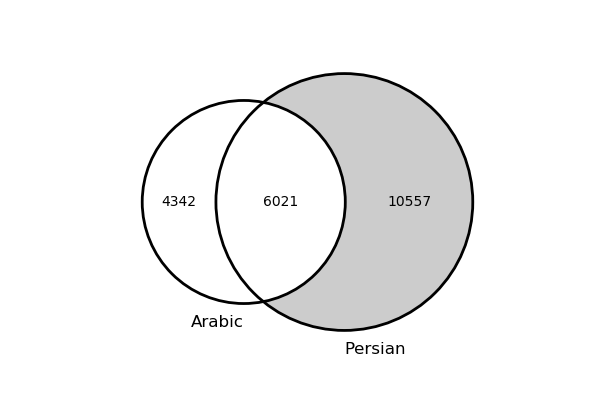
\includegraphics[width=\linewidth]{figures/venn-persian.png}
	\caption[Venn diagram with Persian section highlighted]{Pure Persian works can be identified by querying for works with vocabulary situated largely in the Persian section}\label{fig:venn-pers}
\end{wrapfigure}
\par
The examples above testify to Bah\'{a}'u'llah's ability to avoid words of Arabic origin altogether but they seem exceptional from a linguistic perspective.
Generally His Persian writing is riddled with Arabic vocabulary.
In many cases there are significantly more Arabic than Persian words.
For example, in a letter to Zaynu'l-Muqarrab\'{i}n, nearly eighty percent of the words are of Arabic origin \cite{bahaullah_muntakhabati-az_163}.
There are many other such examples.
In these cases the Persian language is like the mortar holding together the Arabic bricks; the verbs and some of the conjunctions are the only non-Arabic words in the text.
\begin{table}[]
	\centering
		\begin{tabular}{|l|l|r|r|}
			\hline
			\rowcolor[HTML]{EFEFEF}
			\textbf{} & \textbf{File Path}                       & \textbf{Word Count}          & \textbf{Percent Persian}      \\ \hline
1         & bahaullah/text/bahaullah-aiab-176-ar.txt & \cellcolor[HTML]{FFFFFF}1215 & \cellcolor[HTML]{FFFFFF}24.94 \\ \hline
			\rowcolor[HTML]{EFEFEF}
2         & bahaullah/text/bahaullah-st-037-ar.txt   & 441                          & 25.62                         \\ \hline
			\rowcolor[HTML]{FFFFFF}
3         & bahaullah/text/bahaullah-st-154-ar.txt   & 655                          & 21.07                         \\ \hline
			\rowcolor[HTML]{EFEFEF}
4         & bahaullah/text/bahaullah-st-029-ar.txt   & 2450                         & 34.12                         \\ \hline
			\rowcolor[HTML]{FFFFFF}
5         & bahaullah/text/bahaullah-aqa2-6-ar.txt   & 1180                         & 20.76                         \\ \hline
\end{tabular}
\caption{Works of Bah\textbackslash{}'\{a\}'u'llah possibly written exclusively in Arabic }
\label{tab:pure-arabic}
\end{table}
\par
One would not expect the same search strategy to work for revealing pure Arabic works.
The fact that Arabic words are commonplace in the Persian language implies that the vocabulary of most Arabic works would have one foot firmly in the intersection between the two languages.
Roughly 60\% of the Arabic vocabulary also appears in Persian works whereas only 36\% of the Persian vocabulary can be found in Arabic works.
The strategy, however, is quite effective if these circumstances are accounted for and the cutoff is set to a lower threshold.
If it is set at 20\%, for example, 83 works are returned \ref{tab:pure-arabic}.
A cursory review of the supposed Persian vocabulary in these works indicates that it is virtually all Arabic.
\par
Bah\'{a}'u'llah's ability to avoid Arabic words in His Persian writing or write in Arabic without any Persian influences is evidence of His strong command of both languages.
It also suggests that instances in which the two languages intermingle cannot be attributed to a lack of knowledge of either language, as has sometimes been done.
Bah\'{a}'u'llah's writing style changes significantly from one text to another.
These changes are often precipitated by His awareness of His audience.
Failure to account for this fact might lead one to misapply or misinterpret algorithms.
The stylometric methods used to detect author, for example, would be highly suspect even if one could eliminate the paratextual variations and be certain that spaces and letter forms were all effects of the author.
\par
Another example of Bah\'{a}'u'llah's literary awareness and His ability to write with precision can be found in the Hidden Words, a small volume of passages in Arabic and Persian \cite{bahaullah_hidden_2002}.
At the time of the revelation of the Hidden Words (1857) Bahá'u'lláh's audience–--the inhabitants of Baghdad specifically, though it is clear that He had a much wider audience in mind–--would have been divided into four discrete groups: Sunni, Shi'i, Wujudies and Shuhudis.
Each of these, in turn, would be divided into opposing factions: Akhbaris, Usulis, and Shaykhis \cite{lawson_todd_globalization_2005}.
Bah\'{a}'u'llah wrote the Hidden Words in such a way that it would appeal to each faction.
Quotations are woven throughout in paraphrase, there is no mention of a proper name that could signal an allegiance to any faction, no isnads, no legalistic doctrines or cultic pronouncements \cite{lawson_todd_globalization_2005}.
What remains is something that could be seen by all as pure religion.
``A religion apparently unencumbered by the tragedy of history, appearing as a restatement of basic truths through the medium of a compelling religious literary art in both languages of the city: Arabic (71 `verses' and Persian (82 `verses') \cite{lawson_todd_globalization_2005}.''
Such an accomplishment is extraordinary given the sectarian nature of the religious discourse of 19th century Baghdad.
Moreover, it shows a profound awareness of the discourse of each faction; in order to know which words to avoid, Bah\'{a}'u'llah had to be deeply familiar with the discourse of each group.
This work serves as a subtle, yet profound, example of Bah\'{a}'u'llah's linguistic ability and religious knowledge as well as His sensitivity.
It touches upon hundred of religious themes without betraying the sectarian leaning of its Author, demonstrating thereby His intent to elevate the minds of His audience above the prevalent sectarian discourse.
Moreover, it demonstrates an awareness of vocabulary through absence, something the stylometric methods mentioned above cannot do.
The absence of sectarian discourse could not be attributed to anything but intentionality.
\par
A final point worth mentioning is that the Hidden Words seems to have been revealed without solicitation, meaning Bah\'{a}'u'llah was not acquiescing to the request of any individual person.
This is significant for the interpretation of the work in that it represents, perhaps more than other works, the intention of its Author.
In our discussion of the Seven Valleys above we have seen how Bah\'{a}'u'llah, at times, conformed his writing style and subject to the requests of individuals.
The Hidden Words exemplifies His ability to write with precision and avoid sectarian pitfalls.
Each of these points suggests that writing style is not confined to the words of the author.
In the case of the Hidden Words the words that are not used, that clearly could have been used, are also significant.
In the case of the Seven Valleys prior Sufi discourse has a significant influence on the final product.
And in all cases the paratext must be accounted for.
These are examples of the kinds of things that must be considered when applying digital methods to humanities problems.
They should inform the choice of algorithm and the interpretation of outputs.
The fact that they do not transfer across domain supports the claim that local language models are needed in humanistic research.
\section{Conclusion}
It should be clear by now that the application of computational processes to humanities problems should not be casually undertaken.
Each language has its own history that resulted in distinct features that must be accounted for when adopting a language model.
Moreover, literary products---digital or physical---produce the their own paratextual effects capable of distorting the signal of the author.
Closely related to these paratextual effects are the effects of text encoding.
This translation from visual glyphs to computational objects is capable of distorting the signal of the author.
Finally, there are circumstances that are unique to each corpus that must be accounted for when adopting a language model and interpreting the results of any computational study.
In the case of Bah\'{a}'u'llah's writings, His sensitivity to the predilections of His audience combined with the linguistic, cultural, and religious diversity of that audience are responsible for significant shifts in style across His writings.
He frequently employs motifs familiar to His audience resulting in a collection of writings with ties to a plethora of genres and styles.
The position He takes is deliberately linked to past discourse yet unwilling to be subsumed by that discourse.
Given the wide variance in style and vocabulary found in Bah\'{a}'u'llah's writings, significant preliminary work would need to be done to determine the limits of algorithmic inquiry into His style or other questions.
Other areas are worth exploring given that caution is taken to carefully consider the inputs, transformations, and outputs of any chosen algorithm.
\chapter{Word Embeddings}

\chapter{Conclusion}
\newpage
\begin{appendix}
\addcontentsline{toc}{chapter}{Appendices}
\chapter*{Appendix A: Bah\'{a}'\'{i} Published Volumes}
\addcontentsline{toc}{section}{Appendix A: Bah\'{a}'\'{i} Published Volumes}
\label{app-1}
\begin{table}[ht]
	\setlength{\tabcolsep}{18pt}
	\begin{tabular}{ll}
	\textbf{Author} & \textbf{Title} \\
		`Abdu'l-Bah\'{a}	& Majm\`{u}`eh Mon\`{a}jath\`{a} Ha\d{d}rat `Abdu'l-Bah\'{a} \\
	`Abdu'l-Bah\'{a}	& Makat\`{i}b Ha\d{d}rat `Abdu'l-Bah\'{a} Jild 1 \\
	`Abdu'l-Bah\'{a}	& Makat\`{i}b Ha\d{d}rat `Abdu'l-Bah\'{a} Jild 2 \\
	`Abdu'l-Bah\'{a}	& Makat\`{i}b Ha\d{d}rat `Abdu'l-Bah\'{a} Jild 3 \\
	`Abdu'l-Bah\'{a}	& Makat\`{i}b Ha\d{d}rat `Abdu'l-Bah\'{a} Jild 4 \\
	`Abdu'l-Bah\'{a}	& Makat\`{i}b Ha\d{d}rat `Abdu'l-Bah\'{a} Jild 5 \\
	`Abdu'l-Bah\'{a}	& Makat\`{i}b Ha\d{d}rat `Abdu'l-Bah\'{a} Jild 6 \\
	`Abdu'l-Bah\'{a}	& Makat\`{i}b Ha\d{d}rat `Abdu'l-Bah\'{a} Jild 7 \\
	`Abdu'l-Bah\'{a}	& Makat\`{i}b Ha\d{d}rat `Abdu'l-Bah\'{a} Jild 8 \\
	`Abdu'l-Bah\'{a}	&  Maq\`{a}leh Sha\underline{kh}si S\'{i}\'{a}\d{h} \\
	`Abdu'l-Bah\'{a}	&  Muf\'{a}wa\d{d}\'{a}t \\
	`Abdu'l-Bah\'{a}	& Munta\underline{kh}ib\'{a}ti az Makat\`{i}b Ha\d{d}rat `Abdu'l-Bah\'{a} Jild 1 \\
	`Abdu'l-Bah\'{a}	& Munta\underline{kh}ib\'{a}ti az Makat\`{i}b Ha\d{d}rat `Abdu'l-Bah\'{a} Jild 2 \\
	`Abdu'l-Bah\'{a}	& Munta\underline{kh}ib\'{a}ti az Makat\`{i}b Ha\d{d}rat `Abdu'l-Bah\'{a} Jild 3 \\
	`Abdu'l-Bah\'{a}	& Munta\underline{kh}ib\'{a}ti az Makat\`{i}b Ha\d{d}rat `Abdu'l-Bah\'{a} Jild 4 \\
	`Abdu'l-Bah\'{a}	& Munta\underline{kh}ib\'{a}ti az Makat\`{i}b Ha\d{d}rat `Abdu'l-Bah\'{a} Jild 5 \\
	`Abdu'l-Bah\'{a}	& Munta\underline{kh}ib\'{a}ti az Makat\`{i}b Ha\d{d}rat `Abdu'l-Bah\'{a} Jild 6 \\
	`Abdu'l-Bah\'{a}	& Ta\underline{dh}kirat al-Vaf\`{a}' \\
	B\'{a}b & Munta\underline{kh}ib\'{a}t \'{A}y\'{a}t az \'{A}th\'{a}r Ha\d{d}rat Nuq\d{t}eh Awl\`{a} \\
	Baha'u'll\'{a}h & Kit\`{a}b-i-\`{A}qdas \\
	Baha'u'll\'{a}h & Kit\`{a}b-i-\`{I}q\`{a}n \\
	Baha'u'll\'{a}h & Kalim\`{a}t Makn\`{u}neh F\`{a}rs\`{i} \\
	Baha'u'll\'{a}h & Kalim\`{a}t Makn\`{u}neh `Arab\`{i} \\
	Baha'u'll\'{a}h & Majm\`{u}`eh \`{A}lv\`{a}h b`ad az Kit\`{a}b-i-\`{A}qdas \\

	\end{tabular}
\end{table}
\end{appendix}
\singlespacing
\printbibliography
\end{document}
